\section{Solution 1:  Metadata with Special Characters}\label{s:sol1-real}

% \subsection{Metadata Storage}
% 	This solution saves the metadata embedded with the actual data and is stored in
% 	the column family belonging to the actual data. This means that metadata is
% 	included in every super column in a column family as the value of column
% 	\texttt{Metadata}. Since metadata is common for all the entities in an entity
% 	class, every super column contains the same metadata value for this column.For
% 	example, in the University keyspace, metadata in \texttt{Student} is stored in
% 	every super column as seen in Figure~\ref{f:sol1-Student-md}.
% 	
% 		\begin{figure}[H]
% 			\centering
% 			%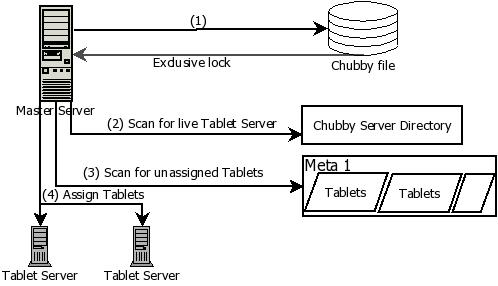
\includegraphics[width=5cm,   height=5cm]{. /figure/random. jpg}
% 			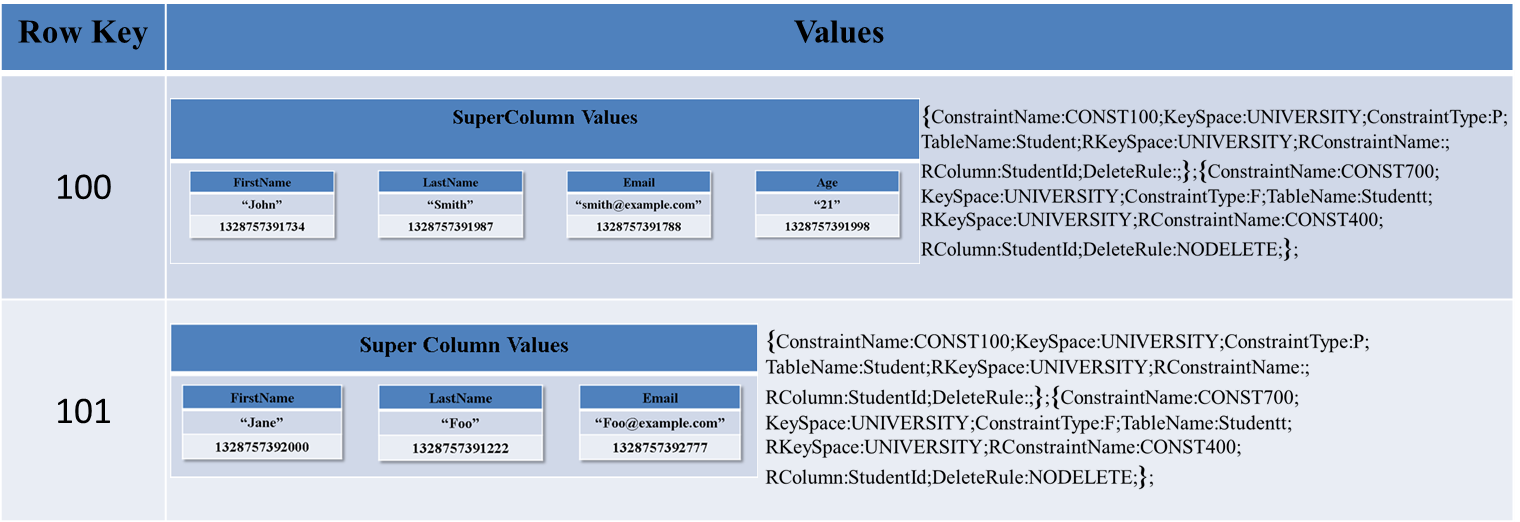
\includegraphics[width=1\textwidth]{./figure/Solutions/Solution1-Student-MD.png}
% 			\caption{Metadata storage in Solution 1}\label{f:sol1-Student-md}
% 		\end{figure}
% 		
% 	In this solution, the structure of the constraints in metadata is as described
% 	in Section~\ref{s:Metadata} and each entity class stores  its \ac{PK}
% 	constraint and related \ac{FK} constraints in the metadata. 
% 	Each entity stores the following constraints as its metadata.
% 	
% 		\begin{itemize}
% 		  \item  \ac{PK} constraint showing the primary key of the column family.
% 		  \item \ac{FK} constraints 
% 				\begin{itemize}
% 					\item In the case of a parent entity the \ac{FK} constraints are the \ac{FK}
% 					constraints of type '\texttt{F}' to identify the child entities when the entity
% 					is being updated or deleted.
% 					\item  In the case of a child entity the \ac{FK} constraint of type '\texttt{R}'
% 					is stored to indicate the parent entities.
% 					\item If an entity is both a parent and a child, then its metadata
% 					stores its \ac{PK} constraint and the \ac{FK} constraints of both types.
% 				\end{itemize}
% 		\end{itemize}
% 		
% 	For instance, \texttt{Student}  is a parent entity with a child dependendent on
% 	it, namely \texttt{Enrolment}. 
% 	Its metadata thus contains its \ac{PK} constraint \texttt{CONST100} and the
% 	\ac{FK} constraint \texttt{CONST700}. Since
% 	\texttt{Enrolment} is a child entity it  stores its \ac{PK} constraint
% 	\texttt{CONST300} and its \ac{FK} constraints \texttt{CONST400} and
% 	\texttt{CONST500}. Similarly, other entities like \texttt{Course} store its
% 	\ac{PK} and respective \ac{FK} constraints.
% 	
% 	Special characters are used within the metadata to separate the constraints and
% 	to identify its different parts. The special characters used in this solution
% 	are '\texttt{\{}', '\texttt{\}}','\texttt{;}' and '\texttt{:}'. The special
% 	characters are used the following way:
% 	
% 	\begin{itemize}
% 	\item Each constraint is enclosed in curly brackets and separated from each
% 	other by the special character '\texttt{;}'. For example,in \texttt{Student}
% 	\texttt{CONST100} and \texttt{CONST700} are enclosed in curly braces and
% 	separated by '\texttt{;}'. Thus, '\texttt{\};}' marks the end of every
% 	constraint in the metadata.
% 
% 
% 	\item The different parts of each constraint are separated by the special character
% 	'\texttt{;}'. For example,  '\texttt{;}' separates the \texttt{ConstraintName}
% 	 and \texttt{Keyspace} and other parts in the constraints \texttt{CONST100} and
% 	 \texttt{CONST700}
% 	 
% 	 
% 	\item Each part and its value are separated by the special character
% 	'\texttt{:}'. For example, \texttt{ConstraintName} is separated from
% 	its value \texttt{CONST100} with a \texttt{:}. This helps in identifying the
% 	name and value for every part while parsing the metadata information
% 	in the \ac{API}.
% 	
% 	\end{itemize}
	
\subsection{Metadata Retrieval/Extraction/Processing}
	In this solution, the metadata is read as a String by the
	\texttt{AbstractEntity} and it is parsed to extract the diffrent parts and its
	values. All the special characters used within the metadata become the
	delimiters for the String parsing and  the different parts and
	its values are converted to tokens. 
	The delimiters used for parsing are:
		\begin{itemize}
		  \item Special characters '\texttt{\{}', '\texttt{\}}' and '\texttt{;}' are
		  the delimiters for extracting each constraint from the metedata.
		  \item Special character '\texttt{;}' is the delimiter for identifying each
		  part within a constraint.
		  \item Special character '\texttt{:}' is the delimiter for extracting the
		  field name and the value from each part of the constraint.
		\end{itemize}
		
	In this solution, an enity class for metadata with the required getter and
	setter access methods is created and used to save the metadata of an entity
	whenevr any operation is invoked on it.
	The \texttt{AbstractEntity} treats metadata just like an entity and sets the
	tokenised values using the metadata entity's setter methods.
	Every time an operation is invoked on an entity the \texttt{EntityManager}
	retreves the metadata from the \texttt{Metadata} column of the entity and loads
	it as text.
		 
	 
	 
\subsection{Metadata Access}
	  
 For referential integrity validation the
	 \texttt{ValidationHandler} accesses each part of the metadata using the
	 relevant setter methods. For instance, to get information of
	the \texttt{DeleteRule} of a constraint on the entity,
	\texttt{ValidationHandler} uses the \texttt{getDeleteRule} method of the
	metadtaa entity class and likewise for all the other different parts
	of the metadata respective getter methods are used.
	 
	 The logic for the referential
	 integrity validation by the \texttt{ValidationHandler} once the String metedata is parsed is the same as described in Section~\ref{ss:VH}.

	In this solution, the metadata is saved  when entities are inserted into the
	column family and thus the metadata is a part of each of the entity.  Since the
	metadata is present as the value in every super column,  accessing the metadata
	information for referential integrity validation is as simple as accessing the
	value itself,  requiring no additional actions or connection to the
	keyspace. Saving the metadata as embedded metadata in this solution is useful
	as entities are replicated across the distributed cluster, making metadata
	easily accessible by every node in the cluster, since it is a part of the
	entity.

	The \ac{API} parses the metadata of an entity by reading any of its
	instances and need not load metadata from any external location.

	On the other hand,  the metadata for an entity would be the same for all its
	instances .  For example,  in the University example,  the metadata
	information for the \texttt{Student} entity is applicable to each of its
	instances,  indicating that each instance  should have a primary key called
	\texttt{StudentID}.
	Similarly,  all \texttt{Course} instances have the same \ac{PK} constraints
	applied on it.  When metadata is saved as a part of the  value,
	every instance of an entity will contain the constraint information
	in it's value.  Since the metadata information and constraints are same for all
	the instances of a single entity ,  this metadata is repeated every time an
	instance of the entity is inserted.  For example,  if
	\texttt{1000} \texttt{Student} instances are inserted,  the metadata for these
	\texttt{1000} instances are saved \texttt{1000} times too, along with these
	instances.  But the metadata is exactly same for all the
	instances \todo{(Figure~\ref{})}.


% 	The distributed nature of cloud \ac{NoSQL} \acp{DBMS} also means that the
% 	metadata is not only repeated several times within the same column family,  but
% 	also across the nodes in the cluster, thus increasing the redundancy of
% 	the metadata.  But such a redundancy and consumption
% 	of space to store the metadata is not a potential issue
% 	in cloud column-oriented key-value \acp{DBMS}, since storage on the cloud is
% 	inexpensive and  does not affect the economic benefits.
% 
% 	Such a storage mechanism is not expected to affect the efficiency of the
% 	cluster negatively as the metadata information is not large in size and is
% 	easily replicated along with the actual data and does not exert any extra
% 	resources in the cluster.  The performance of this solution is analysed  in
% 	Chapter~\ref{}.
% 
% 	Much research has been done in the area of  metadata management in distributed
% 	environments,  where emphasis is laid on the synchronous updates of metadata
% 	storage as well as its efficient storage and access mechanisms(\todo{cite more}
% 	Hackl et al.  2010).
% 	In Hackl et al.  (2010),  metadata management is discussed in the context of
% 	huge file systems, where metadata is stored separately in a suitable \ac{DBMS}
% 	so that such file systems can be managed and administered efficiently without
% 	slowing them down.  To analyse which type of \ac{DBMS} was more suitable for such a
% 	metadata storage,  they conducted various experiments and concluded that
% 	key-value \acp{DBMS} were more efficient in terms of speed,  memory and resource
% 	consumption when compared to popular \acp{RDBMS}.  As a part of their
% 	experiments, they adopted an interesting approach to store metadata in a
% 	key-value \ac{DBMS} ,  namely Tokyo Cabinet,  a popular \ac{NoSQL} \ac{DBMS}
% 	that stores records as simple key-value pairs in data files. Unlike Cassandra,
% 	tokyoCabinet does not involve data types or columns
% 	and so on (\todo{cite}).  In their approach,  metadata about the file system
% 	used in their experiment is inserted as a value which is associated with a unique key and the
% 	different parts of the metadata are separated by semicolons (Hackl et al.  2010).
	